\section{DATCOM Aerodynamics and 6DOF Model}

The third stage increased model fidelity. The equivalent antiship missile geometry was converted into a DATCOM coefficient set, and a section-based mass model was used to estimate CG and inertia for 6DOF simulation.

\subsection{Coefficient Generation}

The workflow preserved the course processing chain:

\[
\texttt{for005.dat} \rightarrow
\texttt{Misdat/RunDatcom2} \rightarrow
\texttt{coeficientes.dat} \rightarrow
\texttt{Coef2Mat} \rightarrow
\texttt{M\_aed.mat}.
\]

The geometry writer was adapted to the Exocet-equivalent missile. The reference point \(X_{ref}=2.700~\text{m}\) was later reused in the 6DOF model as the common moment reference.

\begin{table}[H]
\centering
\caption{Main DATCOM setup values.}
\begin{tabular}{lc}
\toprule
Parameter & Value \\
\midrule
Moment reference & \(2.700~\text{m}\) \\
Diameter & \(0.350~\text{m}\) \\
Nose length & \(0.700~\text{m}\) \\
Center-body length & \(5.090~\text{m}\) \\
Control deflection sweep & \(-20^\circ\) to \(20^\circ\) \\
\bottomrule
\end{tabular}
\end{table}

\begin{figure}[H]
\centering
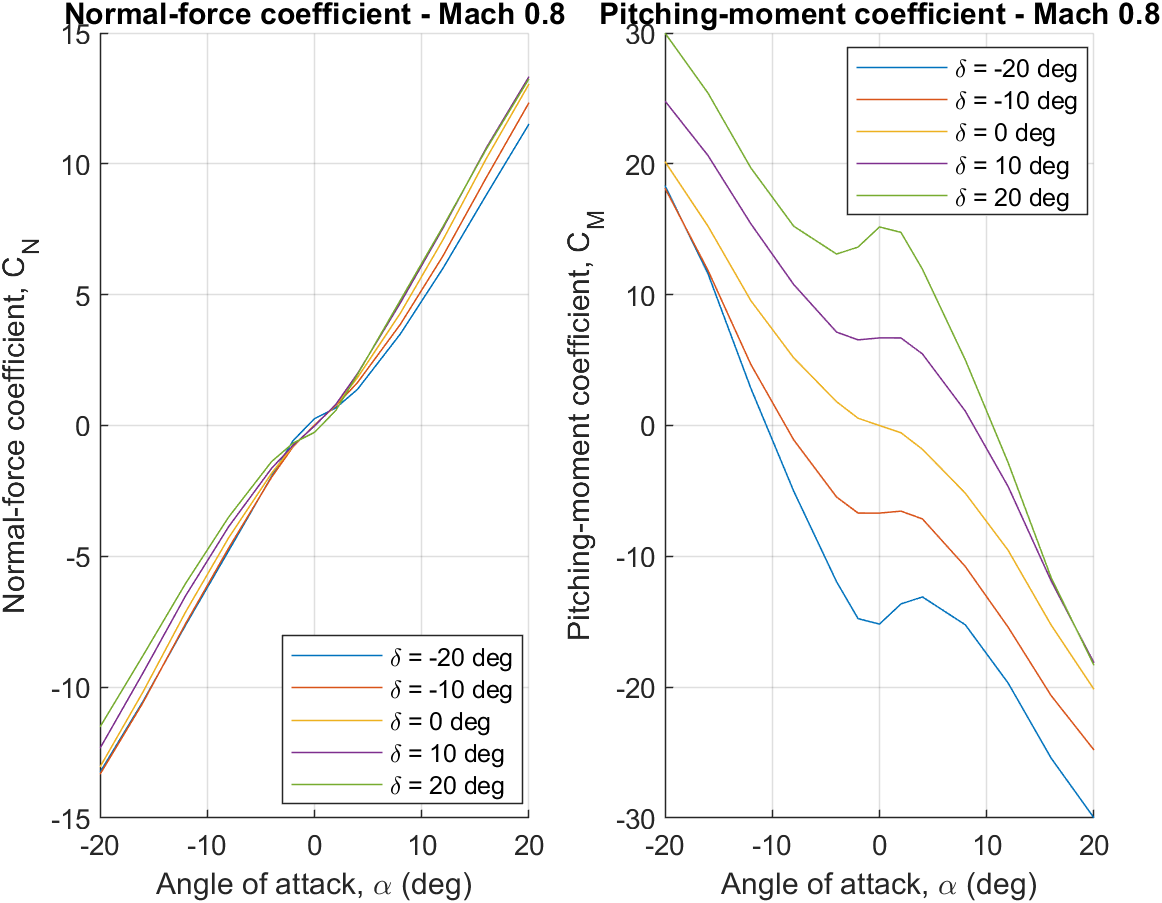
\includegraphics[width=0.78\textwidth]{figures/aero_cm_cn.png}
\caption{Generated normal-force and pitching-moment coefficients.}
\end{figure}

\begin{figure}[H]
\centering
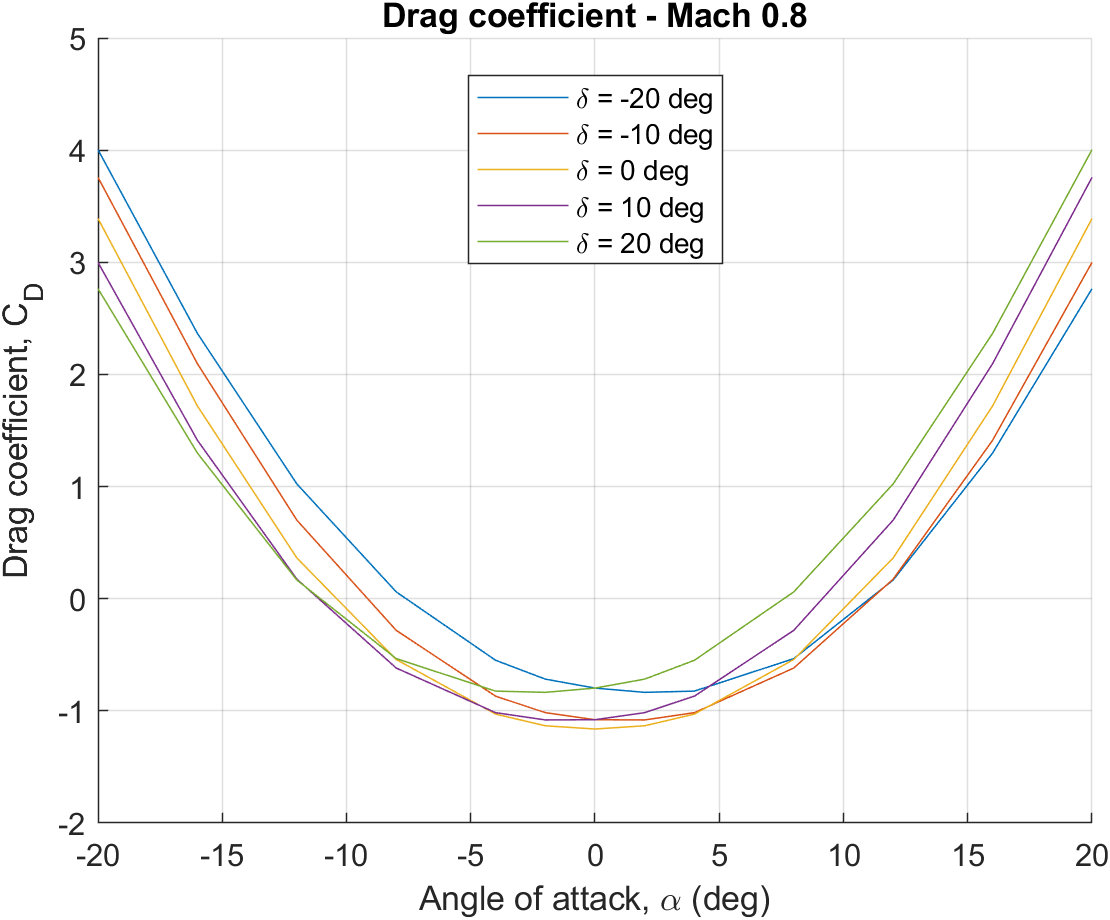
\includegraphics[width=0.78\textwidth]{figures/aero_cd.png}
\caption{Generated drag coefficient.}
\end{figure}

At Mach \(0.9\), \(\alpha=0^\circ\) and \(\delta=0^\circ\), the coefficient set gave \(C_{M\alpha}=-15.36~\text{rad}^{-1}\) and \(C_{N\alpha}=22.70~\text{rad}^{-1}\). The DATCOM value \(X_{CP}=-0.677\) is dimensionless in calibers relative to the moment reference; converting it gives \(X_{CP}=2.937~\text{m}\) from the nose, about \(0.30\) calibers aft of the estimated initial CG. This is consistent with static stability.

\subsection{CG and Inertia}

The missile was divided into control/seeker section, warhead, booster, sustainer and nozzle. The same moment reference used in DATCOM was inserted in \texttt{DadosCGInercia.m}:

\begin{lstlisting}[language=Matlab]
D.CRM = [2.700 0 0]';
\end{lstlisting}

\begin{figure}[H]
\centering
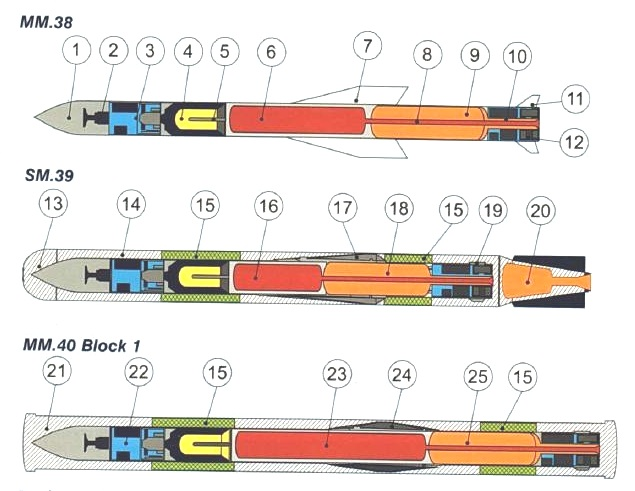
\includegraphics[width=0.9\textwidth]{figures/exocet_internal.jpg}
\caption{Internal subsystem reference used for mass distribution.}
\end{figure}

\begin{table}[H]
\centering
\caption{Initial and final mass properties.}
\begin{tabular}{lcc}
\toprule
Parameter & Initial & Final after burnout \\
\midrule
Mass & \(874.9~\text{kg}\) & \(365.0~\text{kg}\) \\
\(X_{CG}\) & \(2.833~\text{m}\) & \(1.856~\text{m}\) \\
\(I_{xx}\) & \(13.40~\text{kg.m}^2\) & \(5.59~\text{kg.m}^2\) \\
\(I_{yy}=I_{zz}\) & \(2155.40~\text{kg.m}^2\) & \(863.30~\text{kg.m}^2\) \\
\bottomrule
\end{tabular}
\end{table}

\subsection{6DOF Results}

The 6DOF test was a short dynamic check during the initial flight phase, focused on the relationship between control deflection and angle of attack.

\begin{figure}[H]
\centering
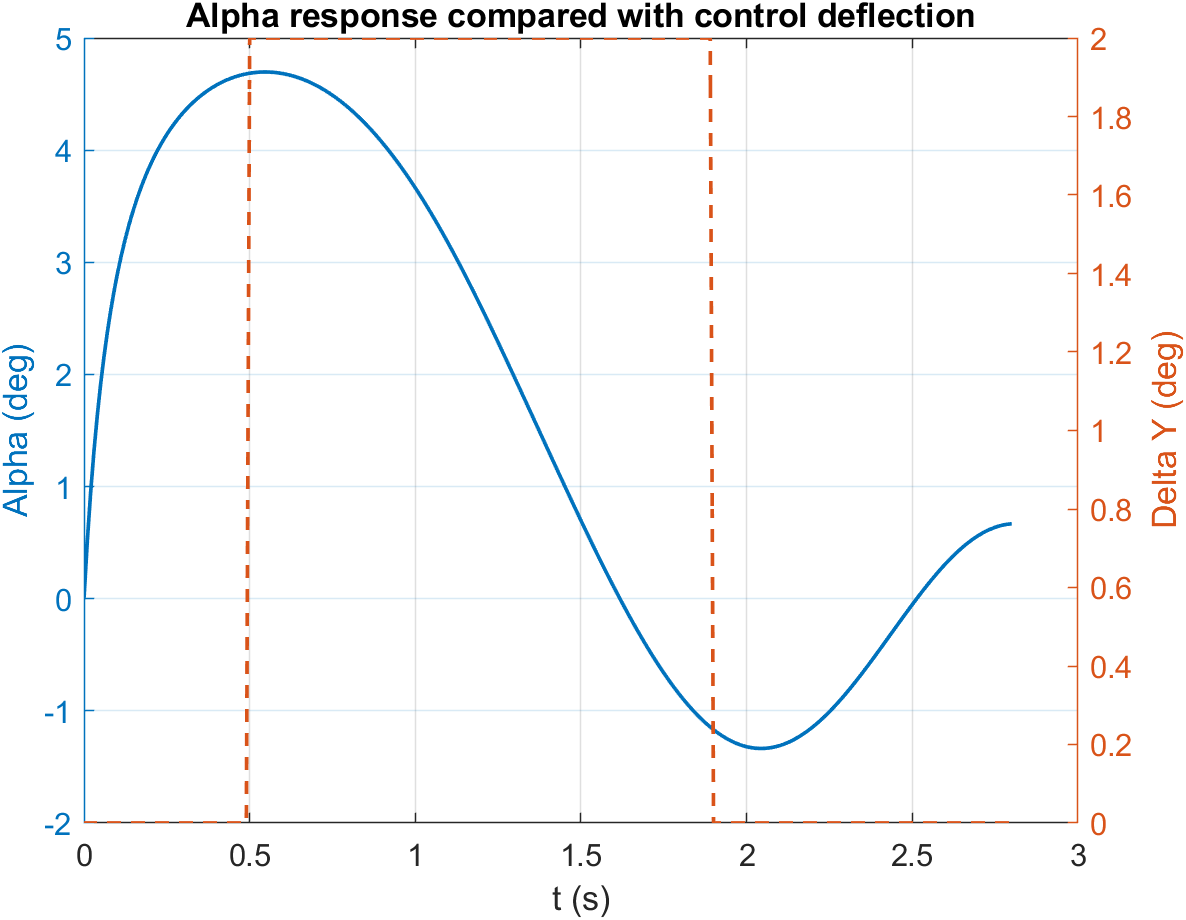
\includegraphics[width=0.86\textwidth]{figures/dof_alpha_delta_overlay.png}
\caption{6DOF comparison between angle of attack and control deflection.}
\end{figure}

\begin{figure}[H]
\centering
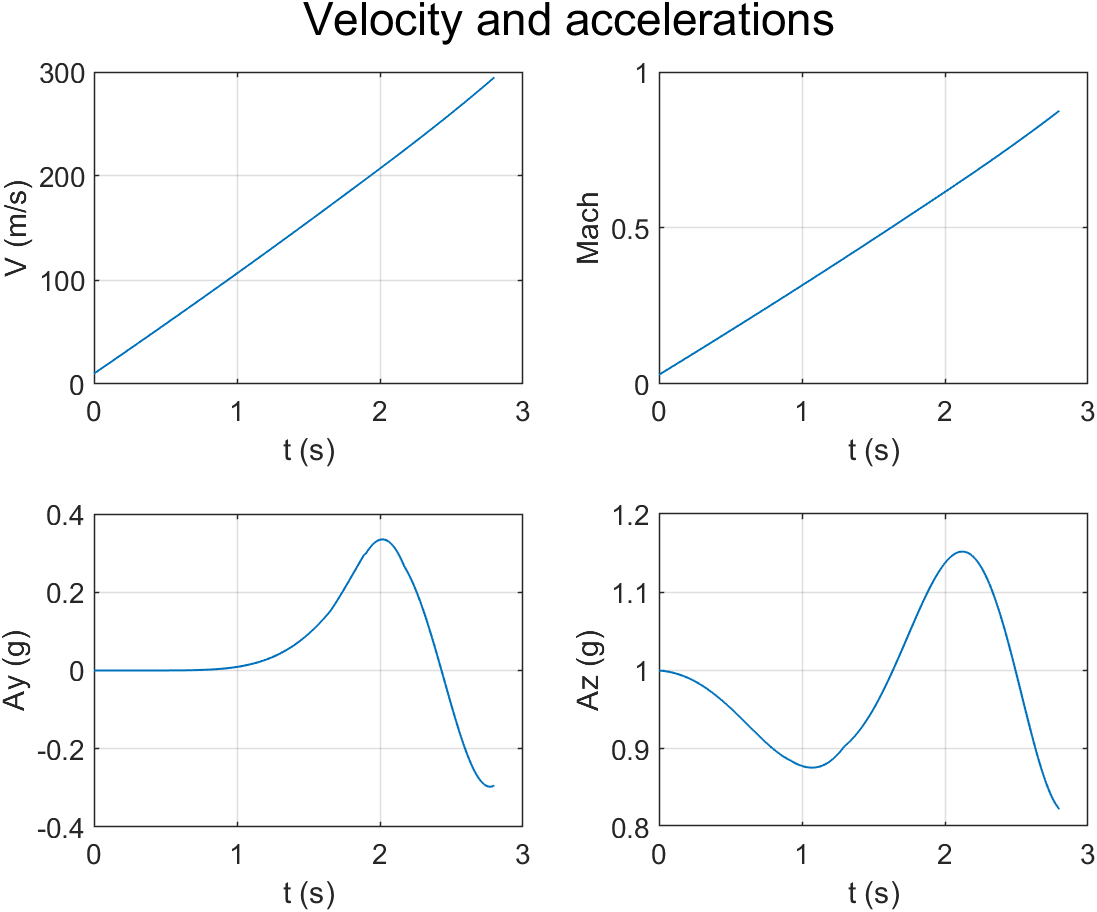
\includegraphics[width=0.86\textwidth]{figures/dof_velocity_accel.png}
\caption{Velocity and acceleration in the 6DOF test.}
\end{figure}

The short simulation served as a consistency check before autopilot design: aerodynamic database, mass properties and 6DOF equations had to respond coherently in the same model.
